

    \item A thermodynamic system is taken from an initial state \( i \) with internal energy \( U_i = 100 \, \text{J} \) to the final state \( f \) along two different paths \( iaf \) and \( ibf \), as schematically shown in the figure. The work done by the system along the paths \( af \), \( ib \) and \( bf \) are \( W_{af} = 200 \, \text{J} \), \( W_{ib} = 50 \, \text{J} \) and \( W_{bf} = 100 \, \text{J} \) respectively. The heat supplied to the system along the path \( iaf \), \( ib \) and \( bf \) are \( Q_{iaf} \), \( Q_{ib} \) and \( Q_{bf} \) respectively. If the internal energy of the system in the state \( b \) is \( U_b = 200 \, \text{J} \) and \( Q_{iaf} = 500 \, \text{J} \), the ratio \( Q_{bf} / Q_{ib} \) is\underline{\hspace{2.5 cm}}.

    \begin{center}
        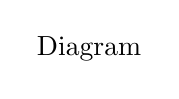
\begin{tikzpicture}
            \node {Diagram};
        \end{tikzpicture}
    \end{center}
    \begin{solution}
        \begin{align*}
            \intertext{Using the first law of thermodynamics, we have:}
            \Delta U &= Q - W
            \intertext{For path \( iaf \):}
            \Delta U_{iaf} &= U_f - U_i \\
            400 \, \text{J} &= Q_{iaf} - W_{af} \\
            400 \, \text{J} &= 500 \, \text{J} - 200 \, \text{J}
            \intertext{For path \( iafb \):}
            U_f &= U_i + (Q_{iaf} - W_{af}) \\
            400 \, \text{J} &= 100 \, \text{J} + (500 \, \text{J} - 200 \, \text{J})
            \intertext{For path \( ibf \):}
            \Delta U_{ib} &= U_b - U_i \\
            100 \, \text{J} &= Q_{ib} - W_{ib} \\
            100 \, \text{J} &= Q_{ib} - 50 \, \text{J} \\
            Q_{ib} &= 150 \, \text{J} 
            \intertext{Next, for path \( bf \):}
            \Delta U_{bf} &= U_f - U_b \\
            200 \, \text{J} &= Q_{bf} - W_{bf} \\
            200 \, \text{J} &= Q_{bf} - 100 \, \text{J} \\
            Q_{bf} &= 300 \, \text{J} 
            \intertext{Thus, the ratio \( \frac{Q_{bf}}{Q_{ib}} \) is:}
            \frac{Q_{bf}}{Q_{ib}} &= \frac{300 \, \text{J}}{150 \, \text{J}} \\
            &= 2
        \end{align*}
    \end{solution}

